\documentclass[10pt,a4paper]{article}
\usepackage[latin1]{inputenc}
\usepackage{amsmath}
\usepackage{amsfonts}
\usepackage{amssymb}
\usepackage{fancyref}
\usepackage{graphicx}
\usepackage{subfig}
\usepackage[all]{xy}
\usepackage{cite}
\usepackage{url}
\usepackage{geometry}
\usepackage{pdflscape}
\usepackage{array}
\usepackage{multirow}
\usepackage{booktabs}
\usepackage{threeparttablex}

\renewcommand{\baselinestretch}{1.25}

%\usepackage[sort&compress]{natbib}
%\graphicspath{ {/home/jordi/Dropbox/INCA/articulo competing risks} }
\author{Jordi Blanch, Ronald B. Geskus, Maria Sala, Xavier Castells, and Montserrat Ru\'e}
\title{Multi-state versus semi-parametric Cox and discrete-time models for assessing the effect of false-positive results of mammogram on breast cancer risk}


\begin{document}

\maketitle
\begin{abstract}
\end{abstract}



\section{Introduction}

\paragraph{}The assessment of breast cancer screening programs traditionally has been based on indicators of performance, e.g. frequency of detected cancers, false-positive results, and interval cancers, obtained cross-sectionally at specific time periods (usually a screening round). Cross-sectional measures are limited, however, by the fact that they do not capture changes over time that may be associated to the risk of developing breast cancer. In contrast, longitudinal studies of women attending breast cancer screening may assess how past and current information on risk factors affect the risk of developing breast cancer.

\paragraph{}In research on breast cancer screening, longitudinal data methods were initially applied to estimate the cumulative rates of false-positive results \cite{Elmore1998, Castells2006, Hubbard2011, Roman2011b, Hofvind2012d}. Later on, longitudinal data analyses have been used to study 1) the frequency of screen-detected cancers over several rounds \cite{Hofvind2006, Blanch2013}, 2) the effect of previous false-positive results on detection rate \cite{VonEuler-Chelpin2012, Castells2013b}, 3) the determinants of interval cancer \cite{Hofvind2006, Blanch2014}, and 4) the association between longitudinal breast density measurements and breast cancer risk \cite{Armero2016}.
Interval cancers are symptomatic cancers that appear between two screening exams or during a period after the last screening exam.

\paragraph{}In a previous work, we studied the determinants of screen-detected cancer and interval cancer  -symptomatic breast cancer that appears after negative tests and before the next invitation \cite{Blanch2014}. We analyzed screen-detected and interval cancers as distinct causes of failure, but, the fact breast cancer is detected in a screening exam precludes an interval cancer, and vice versa. Progression of breast cancer fits better in the multi-state models theory were individuals transition among different health states at variable rates that can be related to their characteristics. 

\paragraph{}Screening for breast cancer may lead to interventions in asymptomatic women, resulting in data on the natural disease course that are observed partially and selective. As a consequence, screening may cause several biases in the analysis of time to event data. In analysis of survival from diagnosis, the most known and studied biases are \textit{lead-time} and \textit{length} sampling. The lead-time is defined as the time gained by diagnosing the disease before the patient experiences symptoms. Even if early diagnosis and early treatment had no benefit, the survival of early detected cancer cases would be longer than the survival of clinical cases. Length sampling bias arises because screen-detected cancers are more likely to have slower growth than non-screen detected cancers \cite{Zelen1969}. In addition, when screen detected and symptomatic cancers are combined, screening may interfere in the assessment of risk factors of breast cancer due to 1) earlier time of detection for screen detected tumours; 2) the fact that symptomatically detected tumours have characteristics that are different from screen detected cancers \cite{Blanch2014}; and 3) there is overdiagnosis of low growth tumours that never would become symptomatic during a woman lifetime \cite{Esserman2013a}. In summary, early detection of breast cancer introduces changes in the natural history of the disease that need to be considered when assessing the effect of interventions or the association of risk factors.

\paragraph{}Simulation models can be used to examine how screening interferes with the assessment of risk factors. Recently, Taghipour \textit{et al.} used a partially observable Markov model to estimate relevant parameters of breast cancer progression and early detection in the Canadian National Breast Screening Study \cite{Taghipour2013}. Previously, other authors had modeled the natural history of breast cancer, using analytic or simulation models that incorporated input data from the literature and made different assumptions \cite{Zelen1969,Chen1996,Shen2001,Lee2003b,Berry2006,Fryback2006,Hanin2006,Lee2006,Mandelblatt2006, Plevritis2006,Weedon-Fekjaer2008a}. The work of the Cancer Intervention and Surveillance Modeling network (CISNET) breast group \cite{Berry2006,Fryback2006,Hanin2006,Lee2006,Mandelblatt2006, Plevritis2006} reflects how modeling studies can provide evidence to complement the results of randomized controlled trials and observational studies. 

\paragraph{}The objectives of this study are 1) To estimate the biases induced by the screening process when assessing the effect of a false positive result in a mammogram test on the progression to pre-clinical cancer and clinical cancer; 2) To evaluate the effect estimates obtained via parametric multi-state models that take interval censoring into account and semi-parametric Cox models or discrete-time models that don't.The paper is organized as follows. Section 2 presents the motivating study, the INCA-CAT,  which contains data on sequential screening mammograms in Catalan women. Section 3 is a methods section that defines concepts relevant to screening, describes the methods used to estimate the effect of false-positive results in previous mammographic exams on the hazard of being diagnosed of breast cancer, and also details how a simulation study was performed. Section 4 presents the results of the simulation study and their application to the INCA-CAT study. Section 5 contains the discussion and conclusions.




\section{Motivating data: the INterval CAncer (INCA) study}
The aim of the INCA study was to assess the determinants of interval breast cancer in women
attending early detection programs in Spain \cite{Domingo2014, Blanch2014}. The INCA study also compared the characteristics associated with screen-detected and interval breast cancers. We selected a subset of the INCA dataset, corresponding to four radiology units of the Catalonia region, the INCA-CAT dataset. 

\paragraph{}Population-based breast cancer screening in Catalonia is offered biennially to all
women aged 50-69 years. Screening mammography has three possible outcomes: 1) negative result
(normal), 2) positive result (abnormal findings requiring further assessments), and 3) early recall
(an intermediate mammogram is performed out of sequence with the screening interval, at 6 or 12
months). Cancers detected at an intermediate mammogram were considered screen-detected cancers \cite{Perry2008}.

\paragraph{}A positive result is considered to be a screen-detected tumour if, after further
assessments, there is histopathological confirmation of cancer. Otherwise, the result is considered
false-positive and the woman is invited again after two years. Further assessments can include
non-invasive procedures (magnetic resonance imaging, ultrasonography, additional mammography) and/or
invasive (fine-needle aspiration cytology, core-needle biopsy and open biopsy). 

\paragraph{}Interval cancer was defined as ``a primary breast cancer arising after a negative
screening episode and before the next invitation to screening or within 24 months for women who
reached the upper age limit" \cite{Perry2008}. This definition was extended until the 30th month, to allow a 6 months margin for women to attend each round. Interval cancers were identified by merging the screening programmes databases with hospital discharge databases and population-based or hospital cancer registries. 

\paragraph{}The INCA-CAT dataset consists of a retrospective cohort of 96,636 women who underwent
mammography exams between January 1, 2000 and December 31, 2006, and were followed-up until June
30, 2009 for interval cancer assessment. These women underwent a total of 230,742 screening
mammograms. During the study period, 963 cancers were diagnosed, of which 671 were detected in screening exams, and 313 emerged as interval cancers. Both invasive and ductal \textit{in situ} (non-invasive) breast cancer carcinomas are included. 

\paragraph{} Among several risk factors studied, the existence of a false positive result in the previous mammogram showed the highest hazard ratio for developing interval cancer, HR=2.71 \cite{Blanch2014}. The corresponding hazard ratio for screen-detected cancer was 1.34. The authors also reported that the effect of a previous false positive result was higher for interval cancers classified as false negative tumours, HR=8.79, than for true interval cancers, HR=2.26.



\section{Methods}
% Especificar com respondrem els dos objectius
% 
% Objectiu principal:
%   - Mètodes: MSM i Cox
%   - Manera: 5 simulacions realitzades
%   - Anàlisi de sensibilitat: amagar informació per reproduir més bé la realitat.
% Objectiu secundari:
%   - Allargem el temps de seguiment fins als 2.5 (o 2) anys per estudiar l'efecte sobre el hazard
%     risc.
%To answer the main objective, we made five simulations with a different features. In each
%simulation, we estimated a Cox model and Markov multi-state models for panel data. To improve
%simulation, we hide some information about the entrance to preclinical or clinical stage. For the
%secondary objective, we uses the same simulation, but we simplify the model to represent a 2 state
%model (healthy, ill) and we study the effect of detect a IC when they occur or in the next
%screening.

\paragraph{}We assume a three-state model 
\begin{displaymath}
\xymatrix @R=0.15cm @C=2cm {
S_0 \ar@{->}[r] & S_p \ar@{->}[r]^{\tau-x} & S_c \\
 & x & \tau \\
}
\end{displaymath}

where $S_0$ indicates absence of breast cancer, $S_p$ indicates the pre-clinical state, where breast cancer is asymptomatic but can be detected with a diagnostic test i.e.\ mammography, and $S_c$ indicates the clinical state or presence of symptoms \cite{Lee1998, Lee2003b}.  The ages at entering $S_p$ and $S_c$ are $x$ and $\tau$, respectively; $\tau-x$ is the sojourn time in $S_p$. 

\paragraph{}The following examples illustrate some possibilities that result from the interaction of the natural history of the disease and the screening process. The times $t_i, i=0,..., n$ indicate when the mammography exams are scheduled. We assume that women attend the exams and that mammogram sensitivity is not 100\%. 

%
\begin{enumerate}
\item Before starting the screening exams the woman enters $S_p$ and then $S_c$. 

\begin{displaymath}
\xymatrix @R=0.3cm @C=0.7cm {
& & t_0 & t_1 & t_2 &   & t_{n-1} & t_n \\
\ar@{-}[rr]|{S_p-S_c} & & | \ar@{-}[r] & | \ar@{-}[r] & | \ar@{-}[r] &  /.../ \ar@{-}[r] & | \ar@{-}[r] & | \ar@{->}[r] & \\
}
\end{displaymath}

This woman is not included in the study because she is diagnosed of breast cancer before the first screening exam at time $t_0$, with the exception of being misclassified because of sensitivity of mammography lower than 100%.
%

\item The woman enters $S_p$ before the first screening exam and enters $S_c$ between $t_0$ and $t_1$. 

\begin{displaymath}
\xymatrix @R=0.3cm @C=0.7cm {
& & t_0 & t_1 & t_2 &  & t_{n-1} & t_n \\
\ar@{-}[rr]|{S_p} & & | \ar@{-}[r]|{S_c} & | \ar@{-}[r] & | \ar@{-}[r] & /.../ \ar@{-}[r] & | \ar@{-}[r] & | \ar@{->}[r] & \\
}
\end{displaymath}

There are two possibilities: a) an early diagnosis at time $t_0$ where age at entering $S_c$ will not be observed; or b) the mammography exam misses the tumour and it is symptomatically diagnosed at time $t$ between $t_0$ and $t_1$. If a) the tumour is screen-detected, if b) it is the type of interval cancer called \textit{false negative}.
%

\item The next example corresponds to the type of interval cancer called \textit{true interval}.
\begin{displaymath}
\xymatrix @R=0.3cm @C=0.7cm {
& & t_0 & t_1 & t_2 & t_3 &  & t_{n-1} & t_n \\
\ar@{-}[rr] & & | \ar@{-}[r]|{S_p-S_c} & | \ar@{-}[r] & | \ar@{-}[r] & | \ar@{-}[r] & /.../ \ar@{-}[r] & | \ar@{-}[r] & | \ar@{->}[r] & \\
}
\end{displaymath}

\end{enumerate}


\subsection{Time scale, censoring, and late entry}
\paragraph{}For the time to $S_p$, two time scales can be chosen: time since entry into the screening program, or age. Age is a more relevant time scale, since it directly reflects the biological process. The incidence of pre-clinical cancer since entry additionally also depends on the study design, i.e.\ at what age women enter the study. For time to $S_c$, the same time scale can be chosen, but it may be of more interest to study the sojourn time, i.e.\ time from $S_p$ to $S_c$. In the multi-state theory, this is called the \textit{clock-reset} approach.

\paragraph{}In the data, the transition $S_0 \rightarrow S_p$ is interval censored. We can assume that the transition $S_p \rightarrow S_c$ is either observed exactly or right censored. When the sojourn time is the estimand, such data have been called doubly (interval) censored. The situation is similar to the estimation of time from HIV infection to AIDS. Typically, HIV infection is not observed exactly but only known to lie in the interval between a last HIV negative test and a first HIV positive test. AIDS is usually either observed exactly or right censored.

\paragraph{}In the INCA study not all women entered the screening program at the age of 50. Women that were above 50 when the program started entered only when they had not yet developed symptoms: they had to be free of clinical cancer. Phrased otherwise, women that already developed pre-clinical or clinical cancer before they would enter the screening program are missed. This may give rise to left truncated data.
  
\paragraph{}Women that have a pre-clinical cancer detected are treated. As a consequence, the clinical cancer will not occur. This implies that transitions $S_p \rightarrow S_c$ are never observed in these women. This is a form of informative censoring for the estimation of the sojourn time distribution. Women with a short sojourn time are more likely to have an interval cancer, i.e.\  to have the clinical cancer observed instead of the screen detected cancer. In fact, if mammography was 100\% sensitive, women that have a sojourn time of more than two years will always be censored at the first screening visit at which the pre-clinical cancer is observed. 

\paragraph{}Estimation of the distribution of age at pre-clinical cancer may still be possible. However, if we use the time of interval cancer as right hand side of the detection interval, the observation times are no longer independent of the event times. An alternative to explore is to set the right hand side at the time at which the first subsequent screening exam would be performed, even though this was not actually done.


\subsection{A Markov multi-state model for breast cancer screening}

\paragraph{}A Markov multi-state model describes how individuals move between a series of states in continuous time \cite{Jackson2011, Geskus2016}. In a Markov model, the next state and the time at which the transition occurs only depends on the present state \cite{Putter2007}. A change of state is called a transition, or an event. Transition intensities that may depend on time $t$, or also on a set of covariates $z(t)$, represent the instantaneous risk or hazard of moving from state $r$ to state $s \neq r$

\[q_{rs}(t;z(t)) =  \underset{\delta t \rightarrow 0} {\lim}\frac{P(S(t+\delta t) = s | S(t) = r, z(t))}{\delta t}.\]

where $S(t)$ indicates the state of an individual at time $t$.


\subsection{Statistical analysis}

\paragraph{} We used three approaches to analyse the INCA-CAT data, 1) the multi-state model, 2) the Cox model, which is the more frequently used in the literature to assess risk factors of breast cancer, and 3) the discrete-time model which also has been used in similar studies \cite{Blanch2013, Ripping2016}.

\paragraph{} When using the multi-state model, we started with a 3-state model and assumed that a) the transition intensity $S_0 \rightarrow S_p$ increases with age, as it does incidence of breast cancer; b) the time at entering $S_p$ is interval censored between the time of a negative exam and the time of breast cancer diagnosis; c) the time at entering $S_c$ is exact for women with IC and is right censored for women with SD cancer; d) there are censored states due to the sensitivity of the mammogram being lower than 100\%; e) false-positive result in the screening mammogram is a time-dependent covariate that is measured as 0 in the absence of a false positive result and 1 from the time of the first false positive result. With this model we estimated the effect of a FP result on the time to entering $S_p$. Then, we considered a 2-state model where the event was BC diagnosis (SC or IC) and compared the effect of FP on BC diagnosis if the IC was detected between screens or in the next screen. The {\tt msm} package for {\tt R} \cite{Jackson2011} was used for the multi-state analyses.

\paragraph{} When using the Cox or the discrete-time models, we also performed different analyses. First, we applied a cause-specific strategy for SD and IC, separately, as in competing risks analysis. For each cause-specific model, the competing event was censored. Second, we considered that the event was breast cancer diagnosis, either SD or IC. We estimated the effect of a FP result in two scenarios, considering the exact age at the IC diagnosis and assuming that the IC cancer was diagnosed in the next screening exam.

\paragraph{} In addition, we conducted a simulation study to explore the performance of the different models for measuring the effect of a false positive result on risk of breast cancer. We were interested in assessing two sources of bias, first the one that arises from the assumptions of the statistical models and then the bias that originates when the statistical models are applied to data only partially observed due to the screening process. We worked with two types of simulated datasets, 1) the \textit{complete data} type which contains all the information on the natural history of breast cancer, and 2) the \textit{observed data} type which contains the partially observed data as a consequence of the screening.


\subsection{Simulation study}

We simulated the natural history of breast cancer as an illness-death model with the three states and transitions $S_0 \rightarrow S_p \rightarrow S_c$. The following assumptions were made:

\begin{enumerate}

\item \textbf{Simulation procedures:} 

For each specific combination of assumptions, the same database of simulated datasets was used to compare the statistical methods of interest. Non-convergence failures were monitored and used to assess if inadequate assumptions were made. The {\tt R} random sampling functions for specific distributions were used to generate the random variables. To enable replication of the datasets, a seed was specified. We simulated 500 datasets with 62,000 women in each dataset. 

\item \textbf{Methods for generating the datasets:} 

\begin{enumerate}

\item \textbf{Time scale}: Age is the time scale with age 50 years as the origin.

\item \textbf{Time to the pre-clinical state, $T_p$}: We assume that it follows a Weibull distribution, We$(\lambda,\nu)$ with $\lambda$ and $\nu$ the scale and shape parameters, respectively, where $h_0(t)=\lambda \nu t^{\nu-1}$ is the baseline risk function of a conventional relative risk model. Times to $S_p$ were generated using the method proposed by Austin \cite{Austin2012, Bender2005} for Cox models.

\item \textbf{Time to study entry, $T_e$}: We will make two assumptions, without and with late entry. For the late entry scenario we assume that the time at entering follows a uniform distribution, $U(0,15)$, and all the data previous to $T_e$ will not be used.

\item \textbf{Sojourn time in the pre-clinical state, $T_s$}: We assume that it follows an exponential distribution Exp(0.25), wich corresponds to a mean time in $S_p$ equal to 4 years \cite{Lee1998}. 

\item \textbf{Time to the clinical state, $T_c$}: $T_c=T_p+T_s$.

\item \textbf{Mammogram sensitivity}: We assume two different values, 100\% and 85\%. We assume that each screening exam is independent within a woman over time.   

\item \textbf{Incidence of false positive results}: We assumed binomial distributions with varying probabilities conditional to the exam sequence number, according to the Rom\'an study \cite{Roman2012}. 

\item \textbf{Effect of false positive results on incidence of breast cancer}:  

The presence of a false positive result will modify the hazard of entering the pre-clinical state according to a relative risks model. Times to $S_p$ were generated using the closed-form expression proposed by Austin \cite{Austin2012} for Cox models with time varying covariates.

\item \textbf{Dropout}: One scenario assumed that dropout occurred randomly during the follow-up. Participation rates of the INCA study at the successive exams were used to generate the dropout. Another, more realistic, scenario assumed that censoring times were associated with false positive results. That assumption was based on evidence that a false positive result produces a decrease in the adherence to screening, and this decrease is more pronounced if the false positive result occurs in the early exams. The RAFP study \cite{Roman2011b}, which included women of similar characteristics as in the INCA study and used a multilevel discrete hazard model, was used to simulate a dropout associated to false positive results.
 
\item \textbf{Number of screening exams}: We assumed two scenarios, four exams as in the INCA study dataset and ten exams as in the majority of the European mass screening programs. We followed-up each woman until the first occurrence of breast cancer diagnosis, administrative censoring at 8 (INCA) or 20 years of follow-up, and dropout during the study.

\end{enumerate}

\item \textbf{Scenarios to be investigated}:
\begin{enumerate}
\item With / without late entry.
\item We fixed the parameters for the Weibull distribution using the INCA-Cat dataset, $scale=0.00025$ and $shape=1.5712$.
\item Hazard ratio of false positive result for time to entering $S_p$, values 1.5 and 4.
\item Dropout: random or related to the false positive results.
\end{enumerate}

\item \textbf{Statistical methods to be evaluated}:
\begin{enumerate}
\item We used the {\tt msm} package in {\tt R} developed by Jackson \cite{Jackson2011} to fit the multi-state models. The {\tt msm} package a) assumes time-homogeneous or piecewise constant hazards. This is a limitation given that we have assumed a Weibull distribution for the time to $S_p$, and an exponential distribution for the sojourn time in $S_p$; b) allows for interval censored transitions and this can be considered a strength of the {\tt msm} package; c) allows for misclassification of states, which is also an asset, given that mammography has sensitivity and specificity lower than 100\%.

\item We estimated the effect of a FP result with the Cox model. We applied a cause-specific strategy for SD and IC, separately. The counting process structure allows to account for left-truncation and time-dependent covariates, as well as non proportional-hazards. We used the {\tt coxph} function of the {\tt survival} package {\tt R}.

\item We estimated the discrete-time model using a logit link for the hazard of the event. The model contains a time indicator variable given by the women's screening participation which acts as multiple intercepts, one per period \cite{Roman2011b}. The time indicator variable represents the baseline logit hazard function \cite{Singer2003}. As in the Cox model, we applied a cause-specific strategy for SD and IC, separately. We considered that the event time corresponds to the last screening participation. We used the {\tt glm} function of the {\tt stats} package in {\tt R}.

\end{enumerate}

\item \textbf{Summary measures of performance}: absolute bias, relative bias (as percentage of the true value), mean square error, and coverage of confidence intervals.
 
 \end{enumerate}

\paragraph{}In each simulation, we focus on quantifying the potential bias due to late-entry and the censoring after detection of pre-clinical cancer. To quantify the bias due to late-entry, we performed two simulations for each scenario, with and without late-entry. The second potential bias is due to the fact that the sojourn time is informatively censored. A woman with a screen detected cancer receives treatment and therefore, it is not possible to observe the time to $S_c$. We assess the effect of not observing the time to $S_c$, when evaluating the effect of a FP result on entering the pre-clinical state $S_p$.

\paragraph{} As a secondary analysis we reduced the three-state model to a two-state model with 1: $S_0$ (absence of breast cancer) and 2: $S_p$ or $S_c$ (breast cancer). Here the time $T$ of interest is age at breast cancer diagnosis (either screen-detected or symptomatically detected). $T$ can be right censored since each women is followed until breast cancer, or end of study. Lost to follow-up is simulated as non-related or related to the false positive status. For clinically diagnosed tumours, we also assessed the effect of extending the follow-up to the next screening exam for estimating the effect of a FP result on the incidence of breast cancer, indistinctly screen-detected or symptomatic.








\section{Results}
\subsection{Simulation study}
In this section we present the results of the simulation study and try to relate the models
performance to their assumptions and to the specificities of the data. For the complete data
analyses we have assumed that there are three states. We assume that women receive 10 biennial
mammographic exams at the age interval 50-69 years, age at entering screening may or may not have
late entry, and the HR of a false-positive result is 2.

\subsubsection{Transition intensities for the three states multistate model. Complete and observed
               data}
Figures \ref{fig:trans_complete} and \ref{fig:trans_observed} present the simulated (theoretical)
and estimated transition intensities in the age interval 50-69 years for the \textbf{complete} and
the \textbf{observed} datasets, respectively. For complete data, the estimated
$S_0 \rightarrow S_p$ piecewise constant transition rates overlap with the theoretical Weibull
function and the estimated $S_p \rightarrow S_c$ transition rate is unbiased (Figure
\ref{fig:trans_complete}). Late entry does not change these results. With observed data, the
estimated $S_0 \rightarrow S_p$ piecewise constant rates follow the Weibull pattern, similarly to
the complete data scenario, but the estimated transition rate overestimates considerably the
theoretical rate (Figure \ref{fig:trans_observed}).

\subsubsection{Hazard ratio of a FP result, for the three state models. Complete data}
Before interpreting the results it is important to mention that the HR of FP for the transition
$S_p \rightarrow S_c$ only can be estimated when using multistate models. We have simulated the
data assuming that a FP result is associated with the transition $S_0 \rightarrow S_p$ with a
$HR = 2$ and it is not associated with the transition $S_p \rightarrow S_c$ (HR=1). For the
multistate model these values are our theoretical values. For the Cox and discrete time models only
the transitions $S_0 \rightarrow S_p$ and $S_0 \rightarrow S_c$ can be estimated. We have assessed
the performance of these models assuming that the theoretical HR value for both transitions is 2.

\paragraph{}Table \ref{tab:HRFP_complete} shows the performance of the studied models, when
considering \textbf{three states} and \textbf{complete data}, with respect to the estimation of the
theoretical HR of having a FP result in the screening mammogram for the transitions
$S_0 \rightarrow S_p$ and $S_p \rightarrow S_c$. The MS3 model performs very well for both
transitions, either \textit{with or without late entry}, with very low bias and coverage higher
than 95\%.

\paragraph{}The Cox CS model has also good properties when estimating the HR of a FP result for the
$S_0 \rightarrow S_p$ transition. For the $S_0 \rightarrow S_c$ the $\overline{\hat\beta}$ value
slightly underestimates the true $\beta$ value with a bias around 2.5\%, independently of the
presence/absence of \textit{late entry}. Coverage is slightly lower than 95\% for the
$S_0 \rightarrow S_c$ transition with \textit{late entry}.

\paragraph{}The discrete time model with three states (DT3) does not perform as well as the MS3 and
the Cox CS models. In this case the percentage bias of the $\overline{\hat\beta}$ associated to the
$S_0 \rightarrow S_c$ transition approaches 5\% and the coverage of the HR intervals for the
$S_0 \rightarrow S_p$ transition is lower than 80\%, for both scenarios \textit{with/without late
entry}.

\subsubsection{Hazard ratio of a FP result, for the three state models. Observed data}
Table \ref{tab:HRFP_observed3} shows the performance of the studied models for the HR of a FP, when
considering \textbf{three states} and \textbf{observed data}. \textit{With or without late entry},
both the MS3 and the Cox CS models perform well in terms of bias, MSE, and coverage. Instead, the
DT3 model shows considerable bias (around 10\% overestimation) and high MSE when estimating the HR
of a FP result for the $S_0 \rightarrow S_c$ transition. The coverage of the intervals for this HR
is lower than 90\% \textit{without late entry} and near 95\% \textit{with late entry} which
probably is due to wide confidence intervals of the estimated HRs as the high MSE indicates.

\subsubsection{Hazard ratio of a FP result, for the two state models. Observed data}
Table \ref{tab:HRFP_observed2} presents the performance of the studied models for the HR of a FP
result, when considering \textbf{two states} in the \textbf{observed data}. Here it is assumed that
the time to the event of interest is the time when the tumour is detected, either by screening or
clinically. We also have assessed the scenario that, for the clinically detected tumours, assumes
that the time to event is the time at the next screening exam. 

\paragraph{}We observe a good performance of the three studied methods, with a better performance
of the multi-state model with \textit{no late entry} followed by the discrete time (DT2 next
screen) and the Cox model (either exact time or next screen). The DT2 exact time model slightly
overestimates the effect and \textit{with late entry} has lower coverage that the other methods. 

\subsection{Aplication to the INCA-CAT study}
Tables \ref{tab:HR3INCA} and \ref{tab:HR2INCA} present the estimates of the HR of false positive
result when applying the models to the INCA-CAT data. 

\paragraph{}When the studied models were applied to the INCA study and the three states $S_0$,
$S_p$ and $S_c$ were considered, the multi-state and the Cox models provided similar estimates for
the HR of FP on the $S_0 \rightarrow S_p$ transition ($HR \approx 1.77$).  However, the
discrete-time model provided a higher estimate of the HR, $1.93$. For the $S_p \rightarrow S_c$
transition, we obtained a HR near to 1 as in the simulation study. The $S_0 \rightarrow S_c$
transitions estimated with the Cox and the discrete time models provide different values, HR around
$1.92$ and $1.22$, respectively.

\paragraph{}When considering only two states, with no distinction between pre-clinical or
clinically detected cancer, all the three models provide similar results, with the HR of a FP
result varying from $1.68$ to $1.73$, when the time of clinically detected cancer is considered an
exact time. When the time of clinically detected cancer is extended up to the next screening exams,
the three estimated values vary from $1.64$ for the multi-state model to $1.82$ for the
discrete-time model.
\clearpage
\section{Discussion}
% + Resum dels resultats
This study assessed the biases induced by early detection on the estimates of the effect of a
mammographic FP result on the progression to pre-clinical and clinical BC. In addition, we
evaluated the effect estimates obtained via parametric multi-state models, which are seldom used in
the screening literature, and semi-parametric Cox models or discrete-time models, which are common
in this area. A simulation study, has provided information on how the assumptions of the
statistical models, or the fact that these models are applied to data partially observed, affect
the parameter estimates. 

% + Comentari dels resultats.
%   - Pq ens surten aquests resultats
\paragraph{}The simulation study showed that, in general, all the models considered had an
acceptable performance for estimating the effect of a FP result, in the different scenarios
assessed. When we worked with three health states, $S_0$, $S_p$ and $S_c$, the multi-state model
showed the best performance in all the scenarios, either for complete or observed data followed by
the Cox cause-specific which had good performance and then the discrete time model with a fair
performance. The simulation analysis of the two state models, also showed a good performance of the
three models considered. The multi-state model with no late entry showed the best performance
followed by discrete-time with time at the next screen for the clinically diagnosed tumours, and
then the Cox model in all the assessed scenarios. Therefore, with simulated data of BC screening,
all the studied models seem good candidates to estimate the impact of a FP result in BC screening 

%   - Resultats per l'INCA. Els he passat a l'apartat de resultats.
\paragraph{}When the studied methods were applied to the INCA study and three states were
considered, the multi-state and the Cox cause-specific models provided similar results for the
$S_0 \rightarrow S_p$ transition, whereas the discrete time model differed from them. When both
pre-clinical and clinical cancers were collapsed, again the multi-state and the Cox model provided
similar results. in this scenario the discrete time model did not differed much from the
multi-state and the Cox models.

% Sobre l'escala del temps
% - MSM i Cox utilitzen l'edat com escala temporal.
% - En canvi, el temps-discret utilitza el número de participacions
% - L'edat és una escala més pròxima al temps 'real' de la malaltia.
% - En canvi, el nombre de participacions suposo que el temps entre
%   participacions ha de ser de dos anys. Però en la vida 'real' no
%   sempre pasa.
\paragraph{}The major difference between MSM and Cox; and discrete-time models are the underline
time. In the MSM and Cox models the underline time is age from 49 years old and the discrete-time
models uses the number of participations as underline time. Age as time is correlated with the real
time of the breast cancer progression. In the other hand, the number of participation is not
correlated with the time of BC progression, because the first participation could be in the 50
years or in the 60 years and the model assume the same risk for all women in their participation.
Also, woman could not come to one participation and the time between participations will be more
than the ``theoretical'' 2 years.

%**** Work in progress ******
%\subsection{Comparison with other studies}
%In the literature of breast cancer screening, there are two main approaches, studies that simulate the screening process to evaluate the impact of screening -as quality of live [Rue], change of analogic to digital mammogram [Comas], overdiagnosis [de Gelder], ...-, or studies that estimate the effect of covariates on the diagnosis of breast cancer -as the effect of a FP result [Castells, Blanch2014, von Euler, Henderson2015], or other variables [Blanch2014, Hofvind2006], screen-detected [blanch, duffy, chen, Uhry, Ripping2016]. We have not found studies that assessed the performance of different methods for estimating the effect of covariates on breast cancer diagnosis in women participating in screening, and taking into account if the cancer was screen-detected or interval cancer.

% En la literatura del cribratge de CM, tenim dos vessants els que simulen el cribratge per evaluar
% algun aspecte (qualitat de vida (Rue), canvi de t`ecnica (Comas), sobrediagn`ostic (de Gelder), entre
% altres) i els que estimen l'efecte sobre el diagostic de CM (efecte del FP (Castells, Blanch2014,
% von Euler, Henderson2015), efecte d'altres variables (p.e. Blanch2014, Hofvind2006), detecci'o
% (blanch, duffy, chen, Uhry, Ripping2016)). No en coneixem cap que estudi quin 'es el millor m`etode
% per a estimar l'efecte sobre la detecci'o del CM segons el m`etode de detecci'o.

%\paragraph{}Some papers in the literature that used multi-state models focused on the estimation of the sojourn
%time in $S_p$ [4 ref]. We have not found any study that used multi-state models to estimate the effect of having a FP result in a previous exam. Some studies estimated the effect of other variables, as history of breast disease, number of births, or family history of breast cancer.
% Els articles que han utilitzat models multi-estat s'han centrat en estimar el temps de
% sojourn [4 ref]. No hem trobat cap que usi aquests models per estimar l'efecte del FP. Sí que s'ha
% estimat l'efecte d'altres variables, com la hist`oria de malaltia mamaria, nombre de fills, hist`oria
% familiar de CM, entre altres.

%\paragraph{}Most of the studies that considered diagnosis of breast cancer in women that participate in screening used the Cox model [ref]. The main limitation of these studies relies on the lack of distinction among screen-detected and interval cancer 
%[von Euler, Henderson2015]. Only a few studies considered if the breast cancer was screen-detected or interval cancer [Hofvind2006,
%Blanch2014].
% La majoria d'articles que estudien la detecci'o del càncer en els programes de cribratge
% han utilitzat models de Cox [ref]. El major problema d'aquest articles és que estudien l'aparici'o
% de càncer sense fer distincions del m`etode diagn`ostic (SCD o IC)[von Euler, Henderson]. Pocs han
% estudiat l'efecte per separat [Hofvind2006, Blanch2014].
%   - Cox CS:
%     - von Euler JNCI
%     - Blanch PlosOne2014
%     - Hofvind 2006 (sobre THS)
%     - Henderson CEBP 2015

%\paragraph{}In the context of breast cancer screening, the discrete-time models were used to estimate the cumulative risk of having a FP result, the adherence of the participants to the screening program or the risk of being diagnosed of breast cancer. Ripping et al estimated the cumulative risk of a FP result, a screen-detected or an interval cancer. In addition, they obtained estimates according to presence/absence of family history of breast cancer.

%Castells et al estimated the risk of screen-detected cancer after observing a FP result in a previous exam. They obtained an estimated OR = 1.81.
% En el context del cribratge de CM, els models de temps discret s'han usat per estimar
% el risc acumulat de tenir un FP, l'adherència de les participants o el risc de detectar un CM.
% Tenim l'article de Ripping2016 on s'estima el risc acumulat de FP, de detectar un CM o de tenir un
% IC. A m'es, separar per si tenen hist`oria familiar o no. Castells et al va estudiar l'efecte de
% detectar un SCD en un cribratge successiu segons si tenia un FP previ (OR = 1.81). 
%   - Discrete-time:
%     - Ripping IJC 2016
%     - Altres hubbard?

% + Limitacions i fortaleses
% + Conclusió final


% There are different approaches in the literature on risk factors of breast cancer. Some authors
% have used Cox models either pooling SD and IC, as in our two-state models, or considering that SD
% and IC are different events and using a cause-specific approach (**** references CS: Blanch2014 i
% Hofvind, S., Møller, B., Thoresen, S., and Ursin, G. (2006). Use of hormone therapy and risk of
% breast cancer detected at screening and between mammographic screens. International Journal of
% Cancer. Journal International Du Cancer, 118(12), 3112-7. http://doi.org/10.1002/ijc.21742 ****).
% Other authors have used logistic regression models comparing IC with SD cancer\cite{Mandelson2000,Ciatto2004,Chiarelli2006,Lowery2011,Blanch2014},
% multinomial models comparing SD, IC, and no cancer (usually the reference group is no cancer)
% % !!! \cite{Blanch2014} No feiem això. No enrecordo cap que tingui aquest plantejament!!! or
% discrete-time survival models estimating the cumulative incidence of SD and IC, separately\cite{Ripping2016}.
% When using logistic regression models IC cancers are compared to SD tumors or both types of breast
% cancer are compared to healthy controls. Breast density \cite{Mandelson2000,Ciatto2004,Chiarelli2006,Lowery2011},
% hormone replacement therapy\cite{Chiarelli2006,Lowery2011}, and other risk factors\cite{Lowery2011}
% are the variables of interest for assessing their association with IC.  
% 
% In general, the authors censor the competing event when estimating the cumulative incidence of one
% of the two events.
% 
% investigated whether breast density increases interval cancer risk in a large sample of women with
% interval and screen detected cancers. They used logistic regression to compare interval with screen
% detected cancers and based their primary analyses on a 24-month screening interval, with a
% sensitivity equal to 72\%. According to the authors, breast density is one of the strongest
% predictors of the failure of mammographic screening to detect cancer. Ciatto et al. \cite{Ciatto2004}
% did a similar study adding healthy controls and also used logistic regression to asses the
% association of breast density and interval cancer.
% 
% 
% Henderson, CEBP 2015 include only FP+TN in the study. They defined
% FP:  mammograms with positive assessment and no cancer diagnosis within one year
% TN: mammograms with a negative assessment and no cancer diagnosis within one year
% TP: mammograms with positive assessment and cancer diagnosis within one year
% FN: mammograms with a negative assessment and a cancer diagnosis within one year
% 
% They consider that cancers associated with TP and FN were assumed to have been present at the time of the screening
% mammogram and their study focused on cancers diagnosed subsequent to the index screening examination. 
% `'We used a partly conditional Cox proportional hazard survival model to assess the association between a false-positive mammography result (with additional imaging or with biopsy recommendation separately) and breast cancer. By using the partly conditional Cox model, we were able to include all mammograms received by an individual woman while accounting for within woman correlation. In these analyses, the mammogram was the unit of analysis. Each false-positive or true-negative mammogram initiated a new follow-up period, which continued until the first of breast cancer diagnosis or censoring by death, end of health plan enrollment (for women in the Western Washington state registry), 10 years of follow-up, or the end of the study period.''


% \subsubsection{Strengths and limitations}
% Afegir que hem usat un patró d'adherència molt sencill. Quan deixa de participar, no retorna.
% Però en la pràctica 'real' succeix i hi poden haver dones que es saltin una participació o varies
\paragraph{}As in most simulation studies, we imposed some restrictive assumptions and we studied
only a limited range of scenarios. In particular, we limited to study one time-depend variable and
affect only one transition. We assumed proportional transition intensities and that subject who
were lost-to-follow-up don't have different risk of BC. Also, we imposed that a woman who missed
one participation don't come back anymore, but in the real-life there are women coming after
missing one participation. Moreover, we assumed that the visit times were independent of the
process, because the visits are scheduled in advance independently of the BC. It is possible that
some breast cancers diagnosed in women that participate in population screening as in the INCA
study are detectable but missed at screening (false negative) and therefore are misclassified as
interval cancers.


% **** Discuss if we change the assumption on sojourn time in $S_p$ if there is a FP result ****.



% \paragraph{Other issues to discuss}
% \begin{enumerate}
% \item Are FP results affecting transition to pre-clinical, sojourn time, stage at clinical
%       detection?
% \item Sojourn time in the pre-clinical state, maybe other distributions (i.e. log-normal) could be
%       assumed. Or, only commented in the discussion.\newline
%       Només a la discussio
% \item Do we introduce diagnostic errors? (sensitivity lower that 100\%, overdiagnosis,...)\newline
%       Hem posat la sensibilitat al 85\%.
% \item Other risk factors (family history, number of live births, menstruation length, other types
%       of breast disease). Also can be commented in the discussion.\newline
%       No ho comentari, ja que no esta en els nostres objectius.
% \item Deaths to causes other than breast cancer. Same.\newline
%       No ho hem tingut en compte
% \item Any distinction between in situ and invasive? In the Canadians study they used only invasive
%       breast cancer.\newline
%       No hem fet diferenciacio. Hauriem de fer un model mes complicat de 5 estats, no?
% \item The Canadians have estimated a mean sojourn time of 3 years for women 50-59. Sensitivity of
%       mammogram was 0.75 for 50-59 yrs.\newline
%       Hem centraria només amb la part de l'efecte del FP, ja que l'objectiu es estudiar l'efecte
%       del FP.
% \item The Canadians use age at entry as a covariate. They justify it in order to take into account
%       how variations in age within age groups affect the transition rates.\newline
%       Si podem l'edat com a covariable, estem suposant que l'inici del cribratge modifica el risc
%       de CM, cosa que no es certa. Per aixo, es millor utilitzar l'edat com a temps de seguiment.
% \end{enumerate}


\subsection{Conclusions}
% Pensar.
This paper suggests that MSM is the best model to estimate the breast cancer progression in the
screening context. To study cancer progression, we do not encourage the use of discrete-time model,
because the time is not related with the progression of BC. Also, we suggest the MSM over
cause-specific Cox, because the SCD and IC are the same diseases in different stage.

Simulation studies based on the real-life scenarios are useful to studies different approaches in
controled environment. So, when we apply the methods in real-scenario, we have tools to interpret
the results and the possible bias.
\clearpage
\section{Tables}

\begin{table}[h!]
\footnotesize
\centering
\begin{threeparttable}
\begin{tabular}{l|c|c|c|c|c|c}
\toprule
\textbf{Method} & \textbf{HR} & \textbf{Parameter} &\multicolumn{4}{c}{\textbf{Performance}\tnote{a,b}} \\ \cline{4-7}
& & & \textbf{Bias} & \textbf{Percentage} & \textbf{Accuracy}  &  \textbf{Coverage}  \\
& & & & \textbf{Bias} &   \textbf{MSE}\\
\midrule
\multirow{2}{*}{\parbox{0.2\textwidth}{MS3, no LE}} & 2 & HR$_{S_0 \rightarrow S_p}$ &0.0043&	0.22& 0.0104	& 97.20\\
& 1 & HR$_{S_p \rightarrow S_c}$ & 0.0010	& 0.10	& 0.0042	&95.80\\
\cmidrule{1-7}
\multirow{2}{*}{\parbox{0.2\textwidth}{MS3, LE}} & 2 & HR$_{S_0 \rightarrow S_p}$ &0.0050&	0.25	&0.0118&	94.80\\
& 1 & HR$_{S_p \rightarrow S_c}$ & 0.0049&	0.49&	0.0046 & 95.60\\
\midrule
\multirow{2}{*}{\parbox{0.2\textwidth}{Cox CS, no LE}} & \multirow{2}{*}{2} & HR$_{S_0 \rightarrow S_p}$ &-0.0203&-1.01&0.0136&	97.20\\
&& HR$_{S_0 \rightarrow S_c}$ &-0.0539&-2.69&0.0173&95.00\\
\cmidrule{1-7}
\multirow{2}{*}{\parbox{0.2\textwidth}{Cox CS, LE}} & \multirow{2}{*}{2} & HR$_{S_0 \rightarrow S_p}$ &-0.0212&-1.06&	0.0154&	95.40\\
&& HR$_{S_0 \rightarrow S_c}$ & -0.0493&-2.47&0.0179&93.40\\
\midrule
\multirow{2}{*}{\parbox{0.2\textwidth}{DT3, no LE}} & \multirow{2}{*}{2} & HR$_{S_0 \rightarrow S_p}$ &-0.0431&	-2.16&	0.0176&	77.60\\
&& HR$_{S_0 \rightarrow S_c}$ &0.0824&	4.12	&0.0239 & 91.60\\
\cmidrule{1-7}
\multirow{2}{*}{\parbox{0.2\textwidth}{DT3, LE}} & \multirow{2}{*}{2} & HR$_{S_0 \rightarrow S_p}$ &-0.0495&	-2.48&	0.0198&	74.80\\
&& HR$_{S_0 \rightarrow S_c}$ &0.1063& 5.18&0.0282&	88.80\\
\bottomrule
\end{tabular}
\begin{tablenotes}\scriptsize
	\item HR: hazard ratio of a false positive result, MS3: multistate models with three states, LE: late entry, CS: cause-specific, DT: discrete time event.
	\item[a] Bias=$\delta=\overline{\hat\beta}-\beta$; Percentage bias=$\left(\frac{\overline{\hat\beta}-\beta}{\beta}*100 \right)$; Accuracy or mean square error (MSE): $(\overline{\hat\beta}-\beta)^2+(\mbox{SE}(\hat \beta))^2$; 	 Coverage:..... 
	\item[b] Assumptions:.....
\end{tablenotes}
\end{threeparttable}
\caption{Simulation results for the complete data. Three state models.}
\label{tab:HRFP_complete}
\end{table}

%\newpage


\begin{table}[h!]
\footnotesize
\centering
\begin{threeparttable}
\begin{tabular}{l|c|c|c|c|c|c}
\toprule
\textbf{Method} &   \textbf{HR} & \textbf{Parameter} &\multicolumn{4}{c}{\textbf{Performance}\tnote{a,b}} \\ \cline{4-7}
& & & \textbf{Bias} & \textbf{Percentage} & \textbf{Accuracy}  &  \textbf{Coverage}  \\
& & & & \textbf{Bias} &   \textbf{MSE}\\
\midrule
\multirow{2}{*}{\parbox{0.2\textwidth}{MS3, no LE}} & 2 & HR$_{S_0 \rightarrow S_p}$ &0.0072&0.36&0.0106&	97.40\\
&1 & HR$_{S_p \rightarrow S_c}$& 0.0186	&1.86&0.0150&	94.80\\
\cmidrule{1-7}
\multirow{2}{*}{\parbox{0.2\textwidth}{MS3, LE}} & 2 & HR$_{S_0 \rightarrow S_p}$ &0.0075 &0.37&0.0123&	94.40\\
& 1 & HR$_{S_p \rightarrow S_c}$ &0.0242&2.42	&0.0153	&94.00\\
\midrule
\multirow{2}{*}{\parbox{0.2\textwidth}{Cox CS, no LE}} & \multirow{2}{*}{2} & HR$_{S_0 \rightarrow S_p}$ &-0.0197 &	-0.98&0.0149& 96.00\\
&& HR$_{S_0 \rightarrow S_c}$ & -0.0233&	-1.51 &0.0479	& 95.80\\
\cmidrule{1-7}
\multirow{2}{*}{\parbox{0.2\textwidth}{Cox CS, LE}} & \multirow{2}{*}{2} & HR$_{S_0 \rightarrow S_p}$ &-0.0211 &-1.06 &	0.0174 &	95.00\\
&& HR$_{S_0 \rightarrow S_c}$ &-0.0152	&-0.76	&0.0477&95.60\\
\midrule
\multirow{2}{*}{\parbox{0.2\textwidth}{DT3, no LE}} & \multirow{2}{*}{2} & HR$_{S_0 \rightarrow S_p}$ & 0.0073	&0.36	&0.0136&	96.80\\
&& HR$_{S_0 \rightarrow S_c}$ &0.1899	&9.49	&0.0974	&87.20\\
\cmidrule{1-7}
\multirow{2}{*}{\parbox{0.2\textwidth}{DT3, LE}} & \multirow{2}{*}{2} & HR$_{S_0 \rightarrow S_p}$ &0.0035&	0.17	&0.0142&	93.60\\
&& HR$_{S_0 \rightarrow S_c}$ &0.2282&	11.41&	0.1119&	94.80\\
\bottomrule
\end{tabular}
\begin{tablenotes}\scriptsize
	\item HR: hazard ratio of a false positive result, MS3: multistate models with 3 states, LE: late entry, CS: cause-specific, DT: discrete time event.
	\item[a] Bias=$\delta=\overline{\hat\beta}-\beta$; Percentage bias=$\left(\frac{\overline{\hat\beta}-\beta}{\beta}*100 \right)$; Accuracy or mean square error (MSE): $(\overline{\hat\beta}-\beta)^2+(\mbox{SE}(\hat \beta))^2$; 	 Coverage:..... 
	\item[b] Assumptions: .....
\end{tablenotes}
\end{threeparttable}
\caption{Simulation results for the observed data. Three state models.}
\label{tab:HRFP_observed3}
\end{table}



\begin{table}[h!]
\footnotesize
\centering
\begin{threeparttable}
\begin{tabular}{l|c|c|c|c|c}
\toprule
\textbf{Method} & \textbf{Parameter} &\multicolumn{4}{c}{\textbf{Performance}\tnote{a,b}} \\ \cline{3-6}
&   \textbf{HR$_{S_0 \rightarrow S_c}$} & \textbf{Bias} & \textbf{Percentage} & \textbf{Accuracy}  &  \textbf{Coverage}  \\
& & & \textbf{Bias} &   \textbf{MSE}\\
\midrule
MS2 exact time, no LE&   & 0.0070&0.35&0.0106	&97.40\\
\cmidrule{1-6}
MS2 exact time, LE&  &0.073&	0.36&	0.0132&	94.40\\
\cmidrule{1-6}
MS2 next screen, no LE & & 0.0064&	0.32	&0.0106&97.40\\
\cmidrule{1-6}
MS2 next screen, LE&  &0.0066 &0.33 &0.0122&	94.40\\
\midrule
Cox exact time, no LE&  &-0.0225&	-1.13&	0.0106&	96.80\\
\cmidrule{1-6}
Cox exact time, LE&  & -0.0216&	-1.08&	0.0122&	95.60\\
\cmidrule{1-6}
Cox next screen, no LE&  &-0.0225&	-1.13&	0.0106&	96.60\\
\cmidrule{1-6}
Cox next screen, LE&  &-0.0216&	-1.08&	0.0122&	95.60\\
\midrule
DT2 exact time, no LE & &0.0497&	2.49&	0.0125	&94.80\\
\cmidrule{1-6}
DT2 exact time, LE&  &0.0565	&2.83 &	0.0147	&92.80\\
\cmidrule{1-6}
DT2 next screen, no LE&  &-0.0035 &-0.17 &0.0095 &97.60\\
\cmidrule{1-6}
DT2 next screen, LE& & 0.0028	&0.14	&0.0109	&95.60\\
\bottomrule
\end{tabular}
\begin{tablenotes}\scriptsize
	\item HR: hazard ratio of a false positive result, MS3: multistate models with 3 states, LE: late entry, CS: cause-specific, DT: discrete time event.
	\item[a] Bias=$\delta=\overline{\hat\beta}-\beta$; Percentage bias=$\left(\frac{\overline{\hat\beta}-\beta}{\beta}*100 \right)$; Accuracy or mean square error (MSE): $(\overline{\hat\beta}-\beta)^2+(\mbox{SE}(\hat \beta))^2$; 	 Coverage:..... 
	\item[b] Assumptions: HR=2 for the $S_0 \rightarrow S_c$ transition.
\end{tablenotes}
\end{threeparttable}
\caption{Simulation results for the observed data. Two state models.}
\label{tab:HRFP_observed2}
\end{table}


\clearpage

\begin{table}[h!]
\footnotesize
\centering
\begin{threeparttable}
\begin{tabular}{l|c|c}
\toprule
\textbf{Model} & \textbf{Parameter} & HR (95\% CI)\\
\midrule
\multirow{2}{*}{MS3} & HR$_{S_0 \rightarrow S_p}$ & 1.7685 (1.2115 - 2.5818)\\ %1.5620 (1.0163 - 2.4007)\\
&HR$_{S_p \rightarrow S_c}$ & 0.9997 (0.5192 - 1.9247)\\%0.6797 (0.3006 - 1.5367)\\
\midrule
\multirow{2}{*}{Cox, CS} & HR$_{S_0 \rightarrow S_p}$ & 1.7722 (1.3389 - 2.3457)\\%1.8500 (1.2920 - 2.6489)\\
& HR$_{S_0 \rightarrow S_c}$ & 1.6152 (1.1207 - 2.3279)\\%0.9507 (0.4467 - 2.0234)\\
\midrule
\multirow{2}{*}{DT3, CS} & HR$_{S_0 \rightarrow S_p}$ & 1.9312 (1.3994 - 2.6120)\\% 1.9488 (1.3243 - 2.7760)\\
& HR$_{S_0 \rightarrow S_c}$ & 1.2223 (0.6333 - 2.1519)\\%1.0742 (0.4499 - 2.1665)\\
\bottomrule
\end{tabular}
\end{threeparttable}
\caption{INCA study: Three state models}
\label{tab:HR3INCA}
\end{table}

\begin{table}[h!]
\footnotesize
\centering
\begin{threeparttable}
\begin{tabular}{l|c}
\toprule
\textbf{Model} & HR$_{S_0 \rightarrow S_c}$  (95\% CI)\\
\midrule
MS2, exact time & 1.6811 (1.1526 - 2.4520)\\%1.4888 (0.9691 - 2.2872)\\
MS2, next screen & 1.6472 (1.1296 - 2.4020)\\%1.4622 (0.9517 - 2.2466)\\
\midrule
Cox, exact time & 1.7051 (1.3643 - 2.1311)\\%1.5878 (1.1489 - 2.1943)\\
Cox, next screen & 1.7099 (1.3696 - 2.1346)\\%1.5632 (1.1317 - 2.1593)\\
\midrule
DT2, exact time &  1.7353 (1.3045 - 2.2705)\\%1.7075  (1.2068 - 2.3505)\\
DT2, next screen &  1.8230 (1.4202 - 2.3112)\\%1.3875 (0.9841 - 1.9018)\\
\bottomrule
\end{tabular}
\end{threeparttable}
\caption{INCA study: Two state models}
\label{tab:HR2INCA}
\end{table}


\clearpage
 \begin{figure}[h!]
\centering
 \subfloat[HR=2]{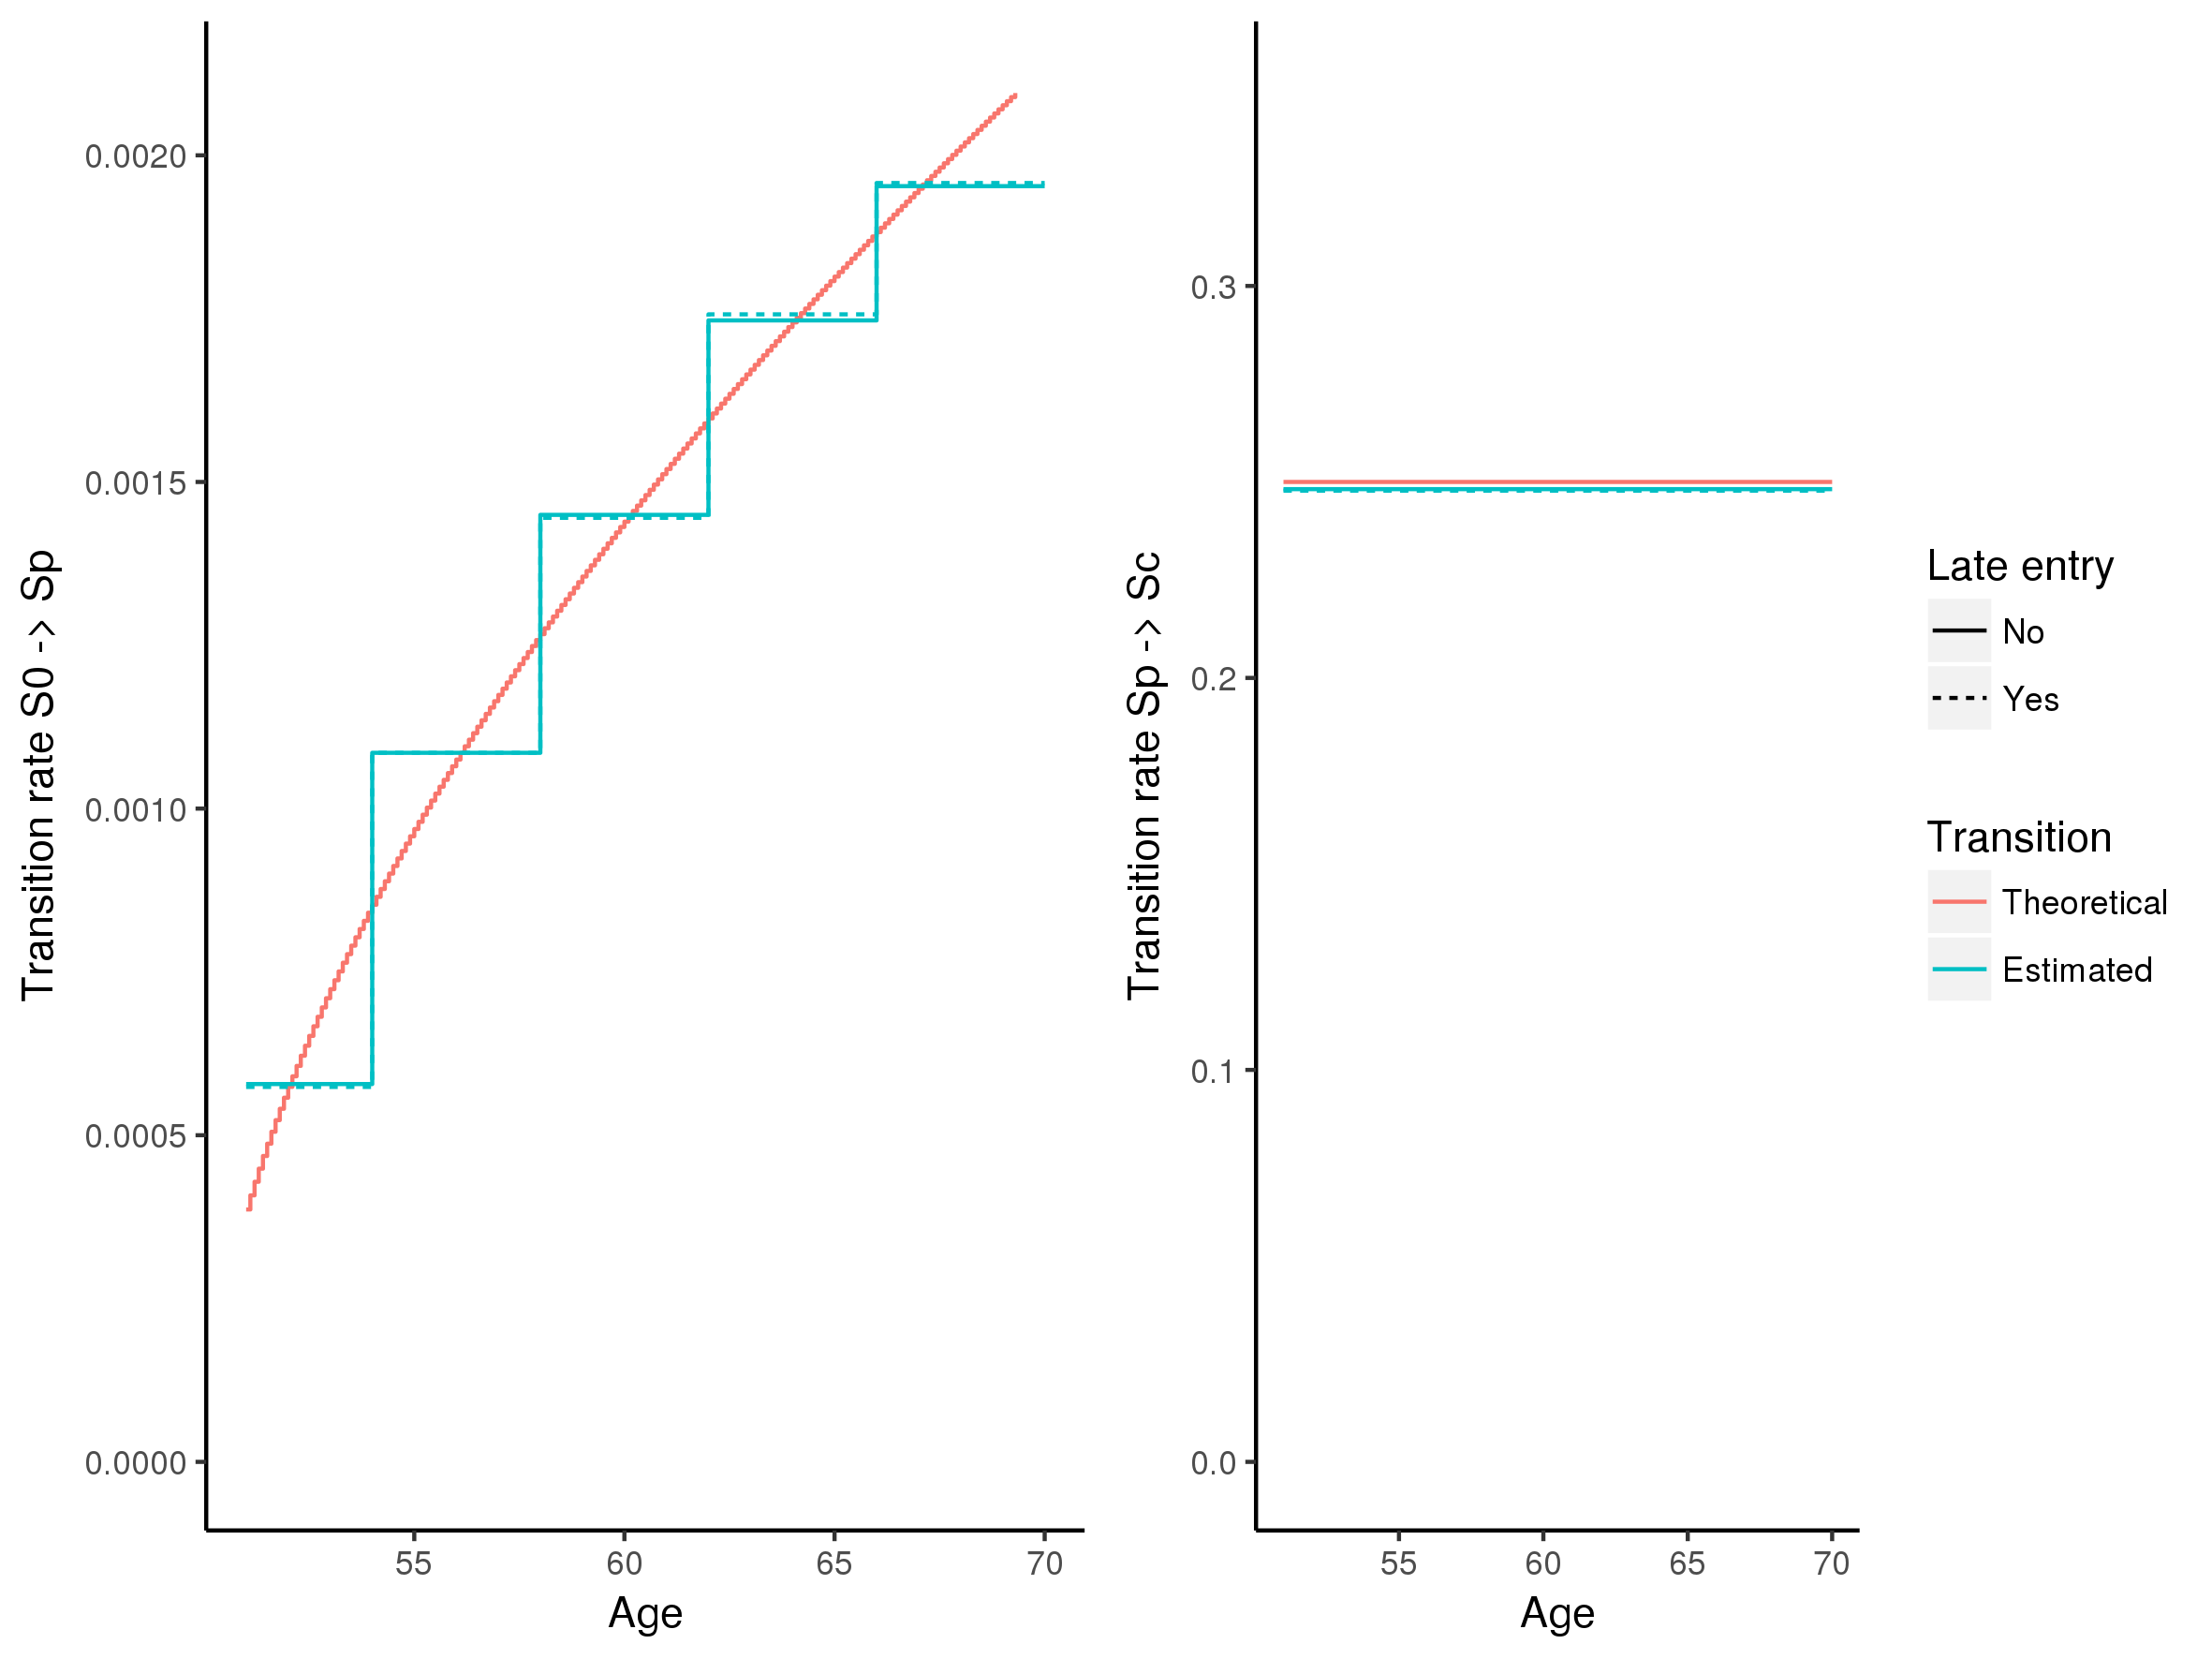
\includegraphics[width=0.7\textwidth]{fig/fig_1.png}}
 %\subfloat[HR=2]{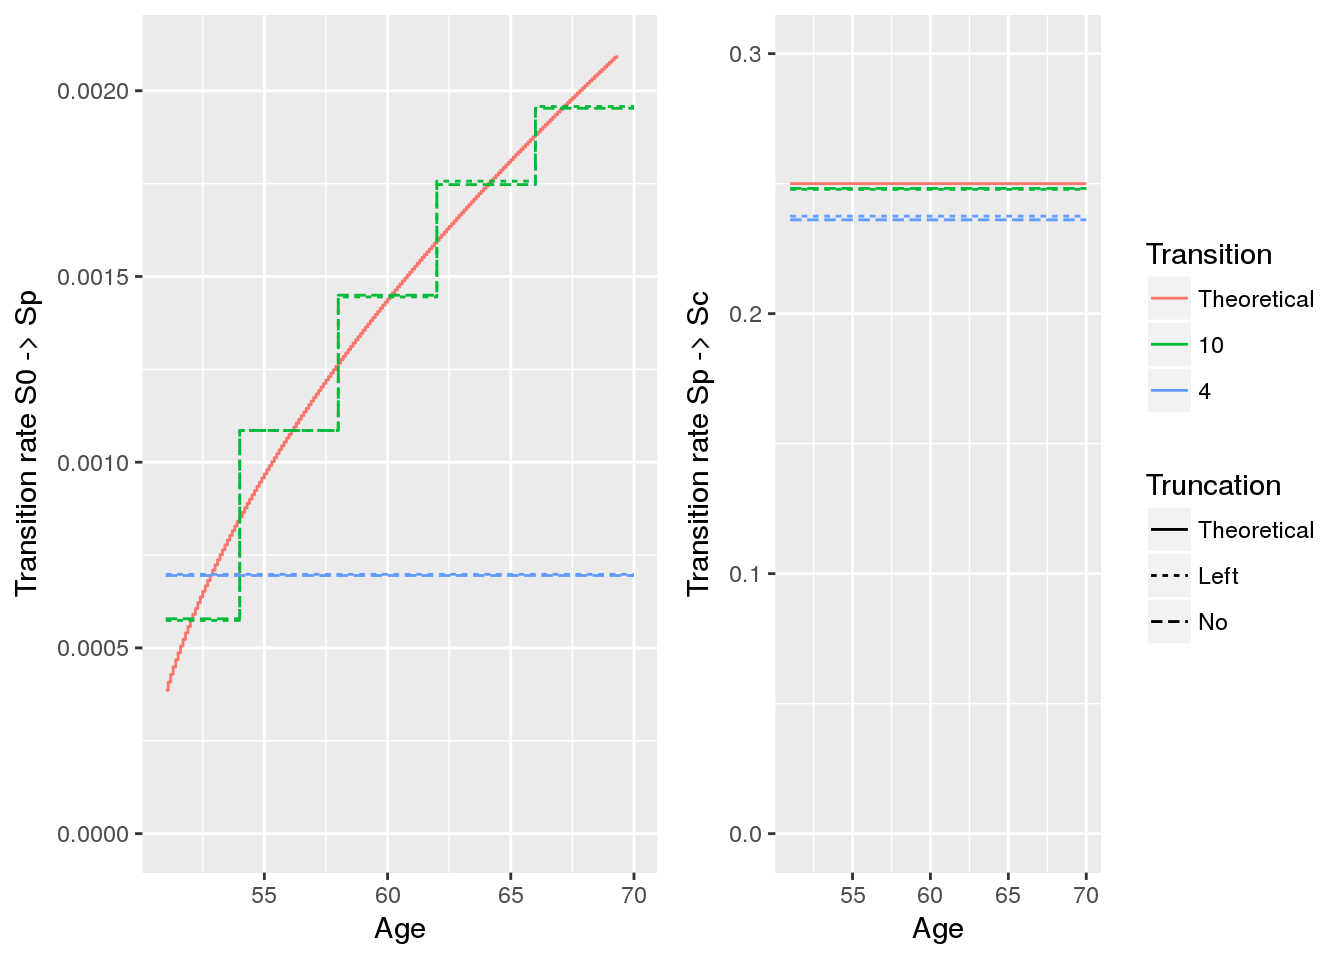
\includegraphics[width=0.7\textwidth]{fig/Fig_com_FP_HR_2.png}}

\caption{Transition intensities for the multi-state with three states (MS3) model. Complete data.}
\label{fig:trans_complete}
\end{figure}

 \begin{figure}[h!]
\centering
 \subfloat[HR=2]{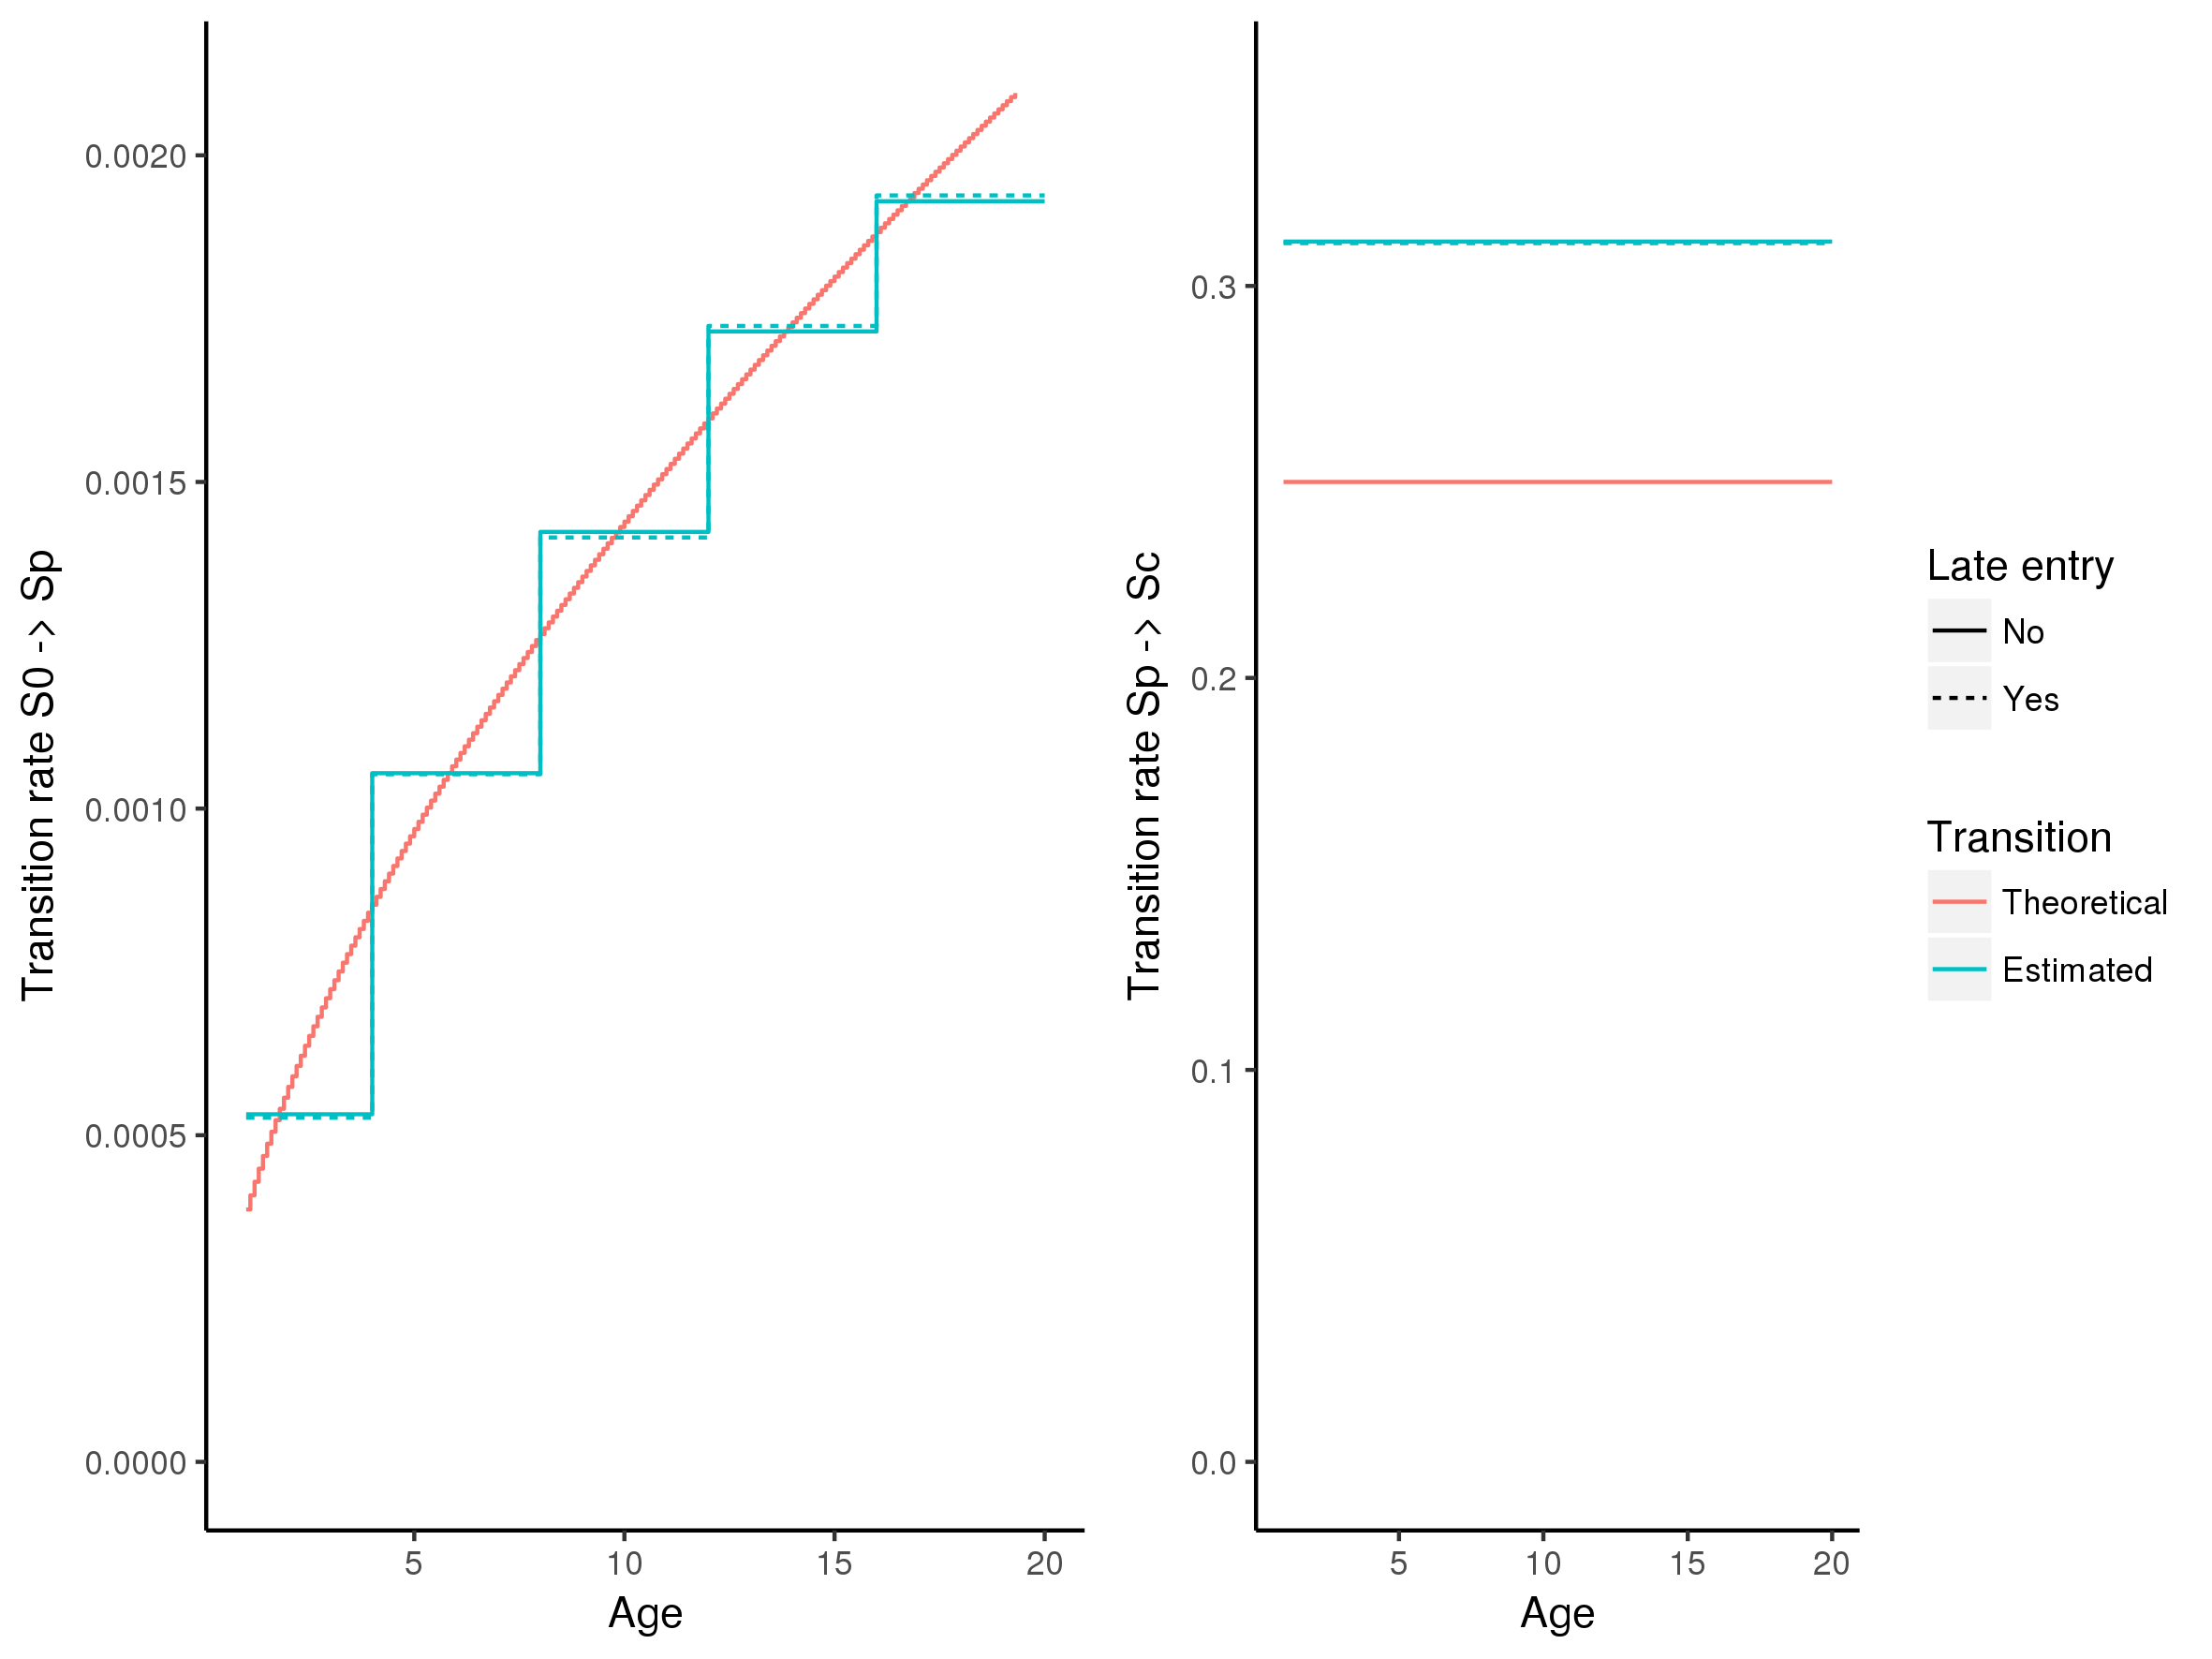
\includegraphics[width=0.7\textwidth]{fig/fig_2.png}}
% \subfloat[HR=2]{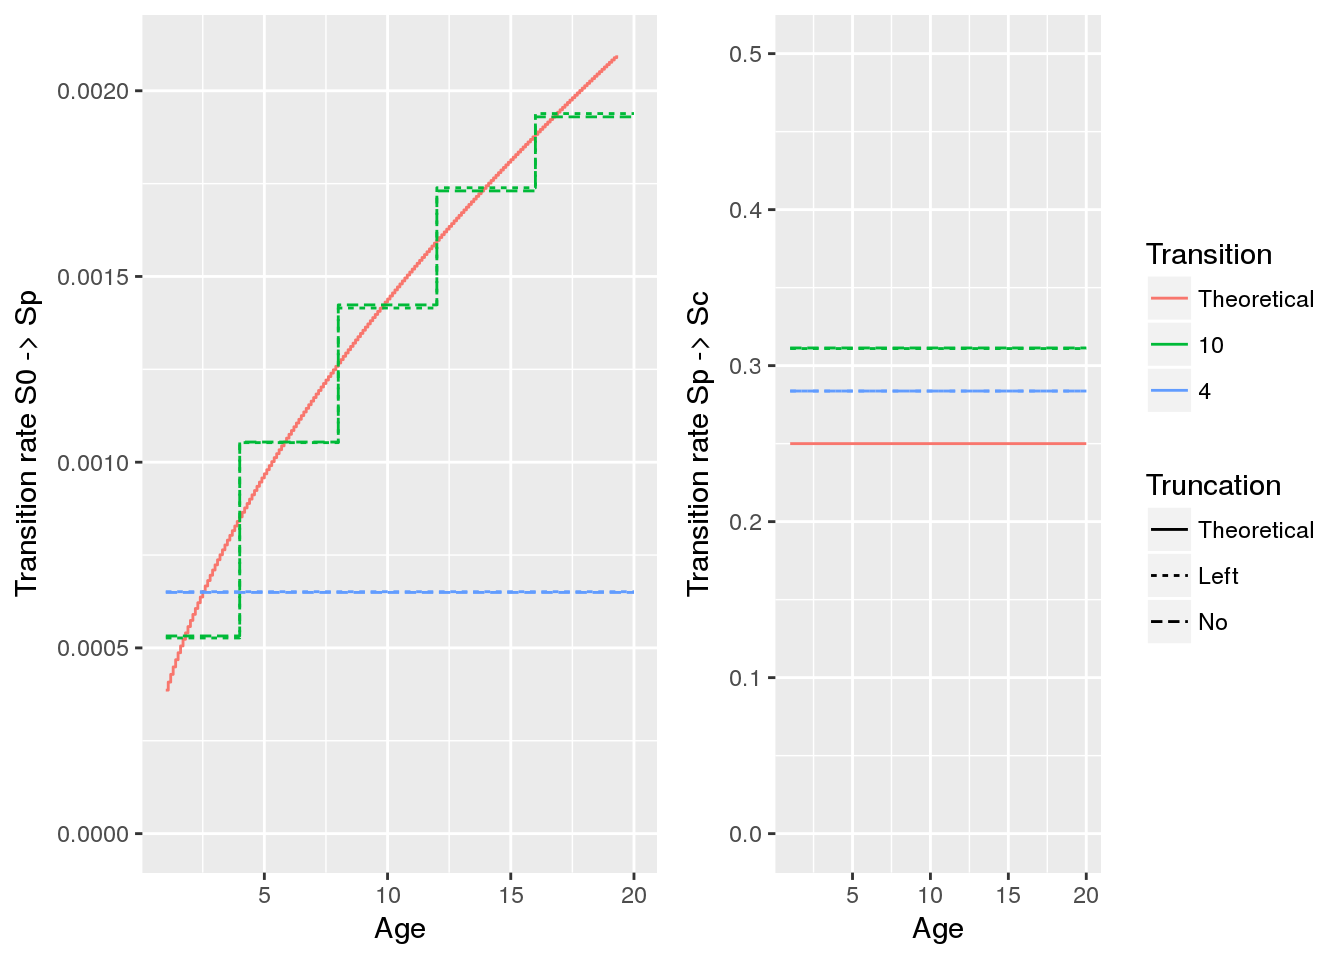
\includegraphics[width=0.7\textwidth]{fig/Fig_obs_FP_HR_2.png}}

\caption{Transition intensities for the multi-state with three states (MS3) model. Observed data.}
\label{fig:trans_observed}
\end{figure}





\clearpage

\section{Acknowledgement}
This paper was supported by the research grant PRX16/00028 from the Spanish Ministry of Education, Culture and Sports, and partially supported by the research grant PI14/00113 from the Spanish Ministry of Economy and Competitiveness and by GRAES-2014-SGR978 from the Generalitat de Catalunya. We thank the researchers of the RAFP and INCA projects for having provided their data.


\noindent {\bf{Conflict of Interest}}

\noindent {\it{The authors have declared no conflict of interest.}}


\newpage

\appendix
\setcounter{table}{0}
\setcounter{equation}{0}
\renewcommand{\thetable}{A.\arabic{table}}
\renewcommand{\thesection}{A.\arabic{section}}
\renewcommand{\thesubsection}{A.\arabic{subsection}}
\renewcommand{\theequation}{A.\arabic{equation}}

\section*{Appendix}



\newpage


\bibliographystyle{wileyj}
\bibliography{bib/blanch}

\end{document} 
